%!TEX root = ../../main.tex
\section{Considerations for RDE Leal}
\label{sec:Considerations for RDE Leal}
\textcolor{red}{
    \begin{myenumerate}
        \item \hypertarget{todo:new title?}{\textbf{TODO:} Not too sure about the title of this section}
    \end{myenumerate}
}
\subsection{Resolution of the Data}
\label{sub:Resolution of the Data}
One of the factors that will affect the parameter values that are obtained from the analysis is the resolution of the data collected \cite{leal2012}.
It is well known that the intensity of higher resolution reflections decay more quickly than lower resolution reflections.
Therefore is the data were collected at a lower resolution the relative intensity throughout the experiment may be expected to be systematically higher than data collected from the same crystal at a higher resolution.
To find out the effect that the resolution dependence would have on the parameter values, the data were scaled to three different resolutions: 1.8\,\AA, 3\,\AA, and 4\,\AA.
The parameter values found for each resolution are given in \ref{tab:RDE params3} and the resulting RDE models plotted with the experimental data are shown in Figure~\ref{fig:Resolution comparison plot - scaled to diff res}.
It is clear that the calculated relative intensity predictions become worse as the resolution of the data decreases.

The other factor that will affect the results of the RDE model are the resolution limits used to perform the RDE Leal integral (equation \ref{eqrdeleal}).
The resolution limits of the BEST data extend from 12345.68\,\AA\ to 0.66\,\AA, thus the integral can be performed between these limits provided the parameter values have been determined.
What is unclear is whether performing the integral to the high resolution BEST limit, 0.66\,\AA, would allow the model to converge to the high resolution relative intensity data despite obtaining the parameter values using low resolution data.
Figure~\ref{fig:Resolution comparison plot - integrated to diff res} shows the RDE models derived from processing the data to the three different resolutions (1.8\,\AA, 3\,\AA, and 4\,\AA) but with the integration performed over the BEST limits.
The magenta, red and green curves correspond to the RDE models using the parameters determined from the data processed to 1.8\,\AA, 3\,\AA, and 4\,\AA\ respectively.
The green and red curves clearly do not converge towards the expected values of intensity decay (blue circles).
The green curve suggests that the crystal is much more resilient than even the 1.8\AA\ data suggests.
The red curve displays an exponential decay shape that is not seen in relative intensity data of crystals at cryotemperatures.
On the other hand the magenta curve looks much more reasonable for the decay of cryotemperature data.

These results suggest that to get the best predictions from the data, it is necessary to collect the data to the highest resolution possible.
Furthermore, if the data are collected to a high enough resolution then calculating the RDE using the \textit{BEST} limits should give a more representative model of the true RDE of the crystal.
This is because the integral is performed over a large resolution range regardless of the diffraction resolution, which will affect the apparent radiation sensitivity.

\begin{table}[ht!]
\small
\captionsetup{justification=centering}
	\caption{Parameter values for Leal \emph{et al.} model determined by the method described in section \ref{sub:Obtaining Model Parameter Values} with data scaled to different resolution limits.}
	\centering
	\begin{tabular}{p{4cm} p{2.4cm} p{2.4cm} p{2cm}}
	\cline{2-4}
		& \multicolumn{3}{c}{Parameter Values} \\
		\hline
		Scaled resolution limit (\AA)			&$B_0$ (\AA$^2$)	  &$\beta$ (\AA$^2MGy^{-1}$) 	 	&$\gamma$ ($MGy^{-1}$)		\\
		\hline
		1.8     													&13.329	    &0.383 			&0.030			\\
		3.0     													&1.190		&0.621  		&0.010			\\
		4.0     													&46.277		&0.536  		&0.006			\\
		\hline
	\end{tabular}
	\label{tab:RDE params3}
\end{table}
\begin{figure}
	\centering
	\begin{subfigure}[b]{1\textwidth}
        \centering
        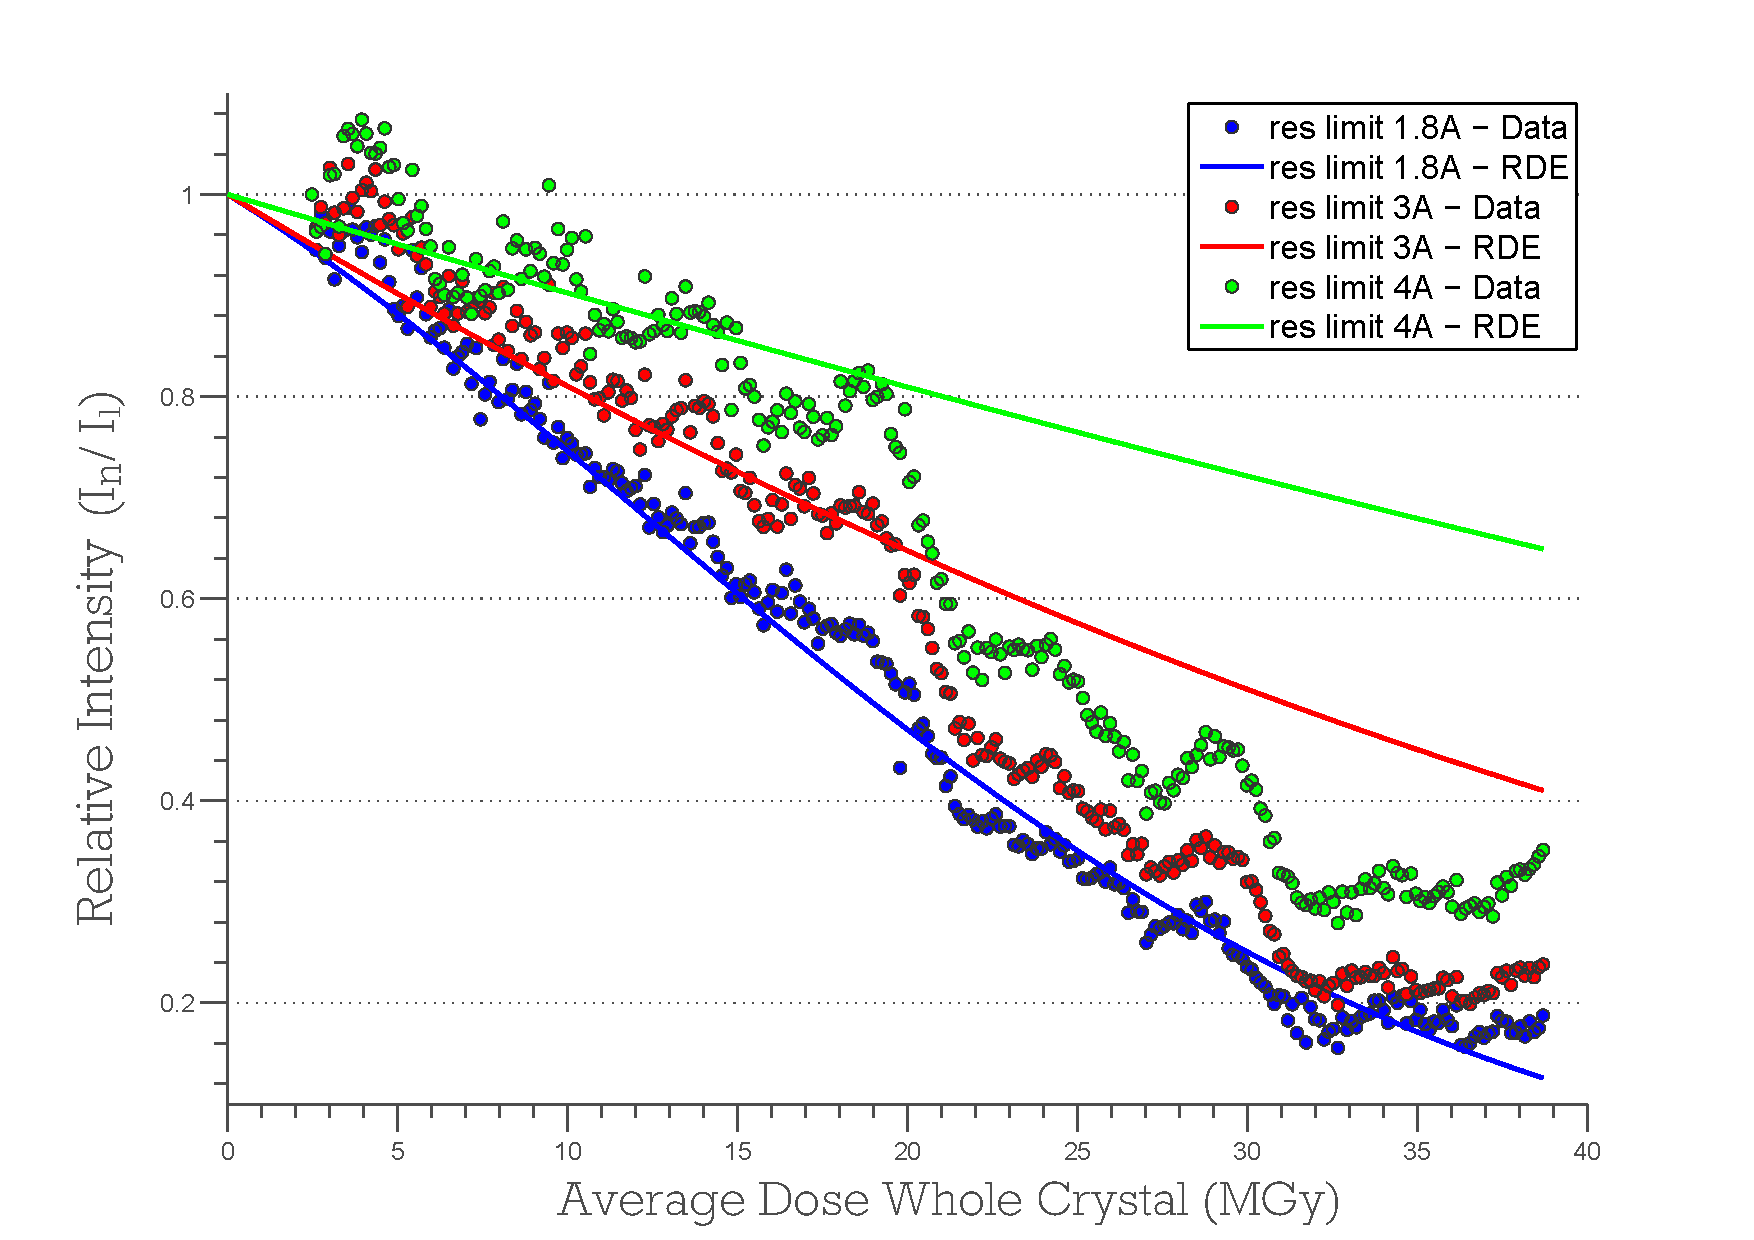
\includegraphics[width=\textwidth]{figures/dwd/rescmpplot1.pdf}
        \caption{}
        \label{fig:Resolution comparison plot - scaled to diff res}
    \end{subfigure}
	\caption{Relative intensity data (circles) plotted with the calculated relative intensity using equation \ref{eqrdeleal}, with the corresponding parameter values for each resolution limit from Table \ref{tab:RDE params3}.}
	\label{figres}
\end{figure}
\begin{figure}
\ContinuedFloat
    \begin{subfigure}[b]{1\textwidth}
        \centering
        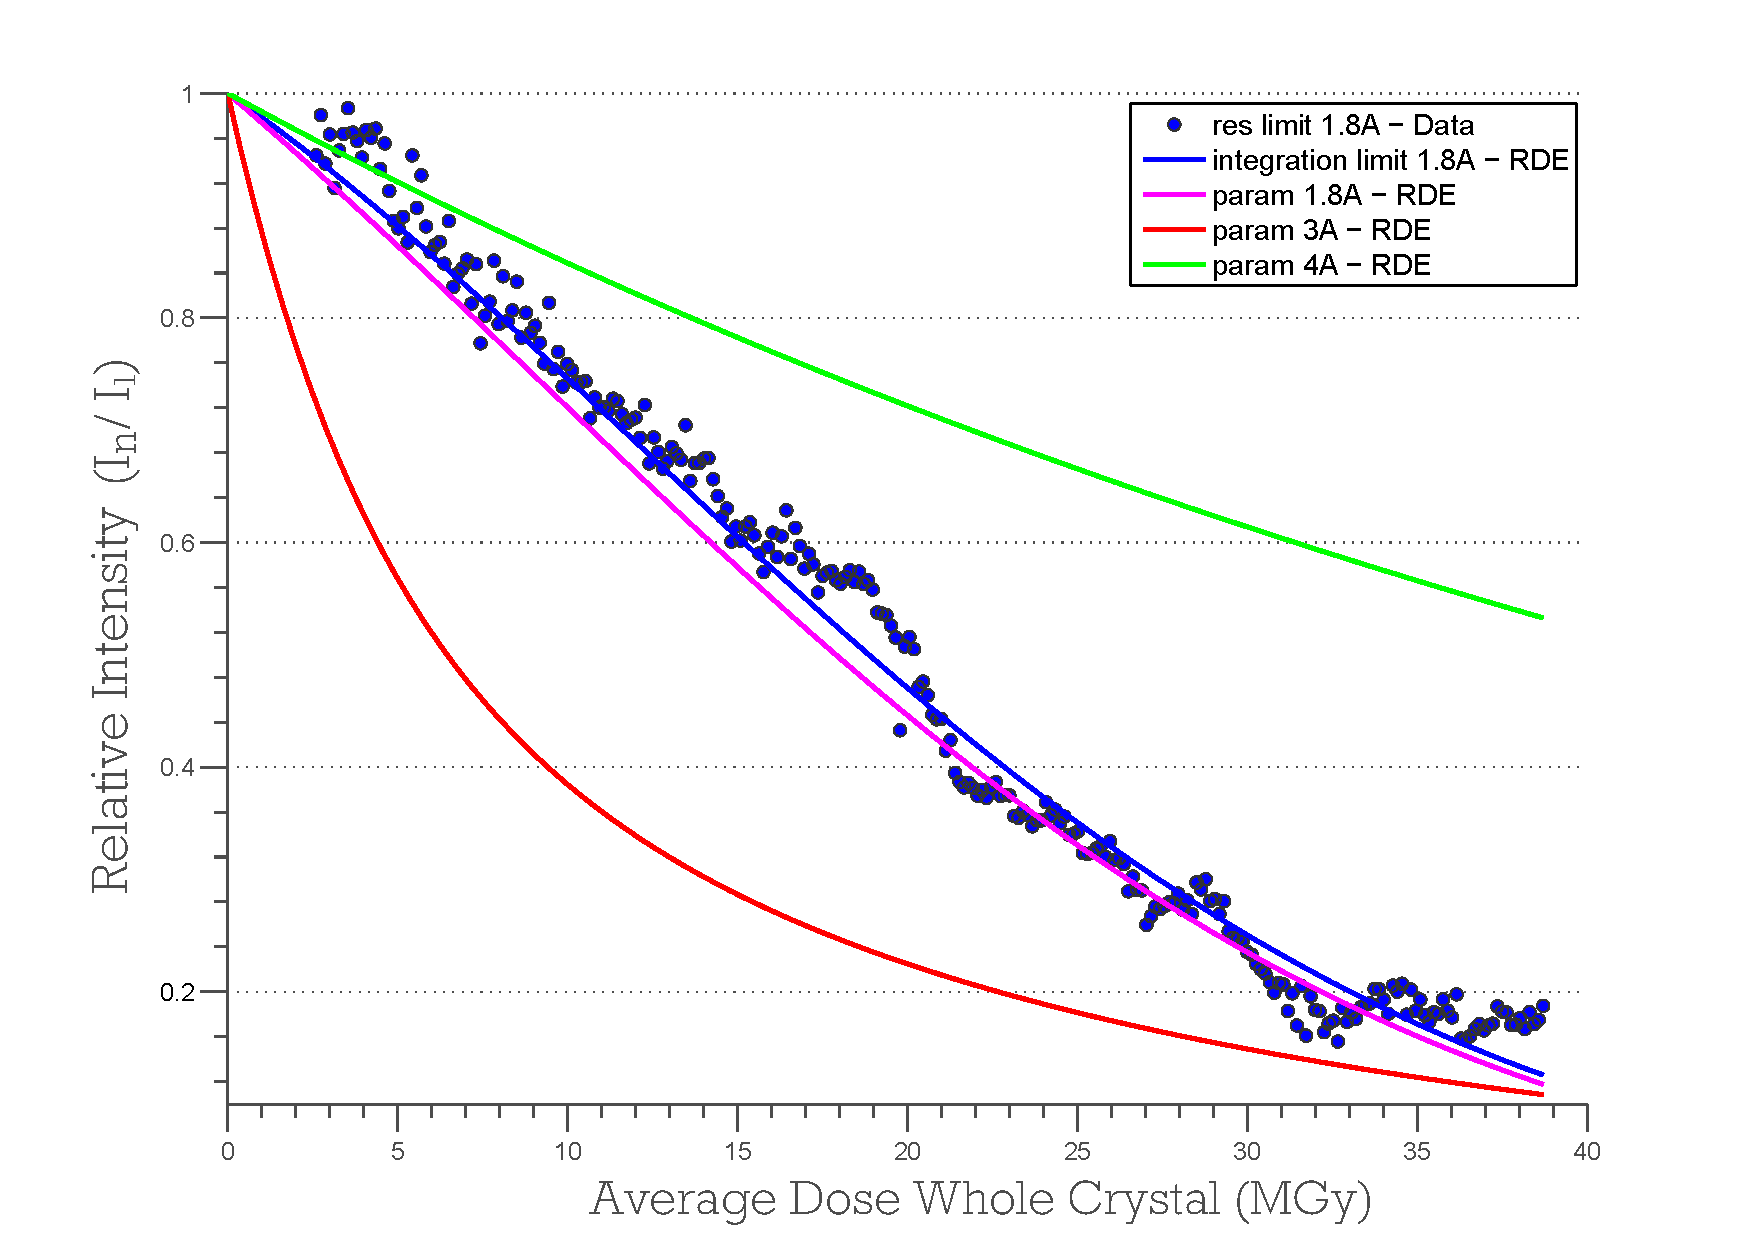
\includegraphics[width=\textwidth]{figures/dwd/rescmpplot3.pdf}
        \caption{}
        \label{fig:Resolution comparison plot - integrated to diff res}
    \end{subfigure}
	\caption{Relative intensities for the data processed to 1.8\,\AA\ (circles) plotted with the calculated relative intensity using equation \ref{eqrdeleal} with the corresponding parameter values for each resolution limit from Table \ref{tabparams3}, but the high resolution integral limit was the limit of the \emph{BEST} intensity data, 0.66\AA. The blue solid line corresponds to the calculated relative intensity value with the high resolution integral limit set at 1.8\AA.}
	\label{figrescont1}
\end{figure}
